\documentclass{article}
%\usepackage[margin=1in]{geometry}
\setlength\topmargin{0pt}
\addtolength\topmargin{-\headheight}
\addtolength\topmargin{-\headsep}
\setlength\oddsidemargin{0pt}
\setlength\textwidth{\paperwidth}
\addtolength\textwidth{-2in}
\setlength\textheight{\paperheight}
\addtolength\textheight{-2in}

\usepackage[english]{babel}
\usepackage[utf8]{inputenc}
\usepackage{fancyhdr}
\usepackage{listings}
\usepackage{graphicx}
\usepackage{xcolor}


\definecolor{codegreen}{rgb}{0,0.6,0}
\definecolor{codegray}{rgb}{0.5,0.5,0.5}
\definecolor{codepurple}{rgb}{0.58,0,0.82}
\definecolor{backcolour}{rgb}{0.95,0.95,0.92}


\usepackage{booktabs}
\usepackage{pgfplotstable}



\lstdefinestyle{mystyle}{
	backgroundcolor=\color{backcolour},
	commentstyle=\color{codegreen},
	keywordstyle=\color{magenta},
	numberstyle=\tiny\color{codegray},
	stringstyle=\color{codepurple},
	basicstyle=\ttfamily\footnotesize,
	breakatwhitespace=false,
	breaklines=true,
	captionpos=b,
	keepspaces=true,
	numbers=left,
	numbersep=5pt,
	showspaces=false,
	showstringspaces=false,
	showtabs=false,
	tabsize=2
}
\lstset{style=mystyle}

\title{Machine Learning Project 3 Neural Networks}
\author{Yifeng Qin, Pedram Safaei}
\date{November 8th}

\begin{document}

\maketitle

\section{calculate\_loss(model, X, y)}
To calculate the loss we need to find the y hat to give to the softmax and cross entropy functions. We created a helper function (calculate\_helper\_variables(model,X, h\_flag = False)) that calculates the helper variables described in the project description. \newline 
\begin{lstlisting}[language=Python]
	def calculate_helper_variables(model,X, h_flag = False):
    a = np.dot(X, model["W1"]) + model["b1"]
    h = np.tanh(a)
    z = np.dot(h, model["W2"]) + model["b2"]
    if h_flag:
        return z,h
    return z
	\end{lstlisting}
	
This helper function will return the z helper variable and h if the h\_flag is set true. We first calculate the helper variable a. It is found by taking X(training data) and dotting it with W1 and b1 which are the weights and bias. To calculate h, we take the helper a variable and pass it to the tanh which is our activation function to calculate the output. To calculate the z helper variable we take the calculated h value and dot it with the W2 added to b2. In calculate\_loss(model, X, y) we set the helper variable z by calling the helper function. Then we calculate the y hat where the z value is passed to the softmax function to give us the prediction. The y hat and y label will be passed to cross entropy loss function. There it will sum over our training examples and add to the loss if the prediction is incorrect. The function will return the loss by multiplying it by -1 over the number of samples.

\begin{lstlisting}[language=Python]
	def calculate_loss(model, X, y):
    Loss = 0
    radius = y.shape[0]
    z = calculate_helper_variables(model,X)
    y_hat = np.exp(z) / (np.sum(np.exp(z), axis=1)).reshape(-1, 1)
    for i in range(radius):
        Loss = Loss + np.log(y_hat[i][y[i]])
    return (-1/radius) * Loss
	\end{lstlisting}

\section{predict(model, x)}
The prediction function is very similar to the loss function. Instead of taking in the whole training data, it will be passed one sample without the label. To calculate the y hat we will call the helper function (calculate\_helper\_variables(model,X, h\_flag = False) to give us our z helper variable. The softmax function will find the ratio of the exponential of the z value and the sum of exponential z values. All the probabilities will be between 0 and 1 and the sum of them all will come out to 1. The function will then append all the predictions into a list and return that list. 

\begin{lstlisting}[language=Python]
	def predict(model, x):
    Prediction = []
    z = calculate_helper_variables(model,x)
    y_hat = np.exp(z - np.max(z)) / (np.exp(z - np.max(z))).sum()
    for i in y_hat:
        Prediction.append(np.argmax(i))
    return np.array(Prediction)
	\end{lstlisting}
	

\section{build\_model(X, y, nn\_hdim, num\_passes=20000, print\_loss=False)}
This function is where all the training happens. For every epoch, which is the num\_passes in this case we will predict all the features, run gradient decent and propegation and output the loss if necessary. According to the project description model is supposed to be a dictionary hence all weights and biases are saved in the model dictionary and it will get populated at the beginning of the build model using the initialize function (helper function so it was not included, refer to the program for more info)
	
\noindent Then we will run through a for loop that runs for the number of passes that were entered. First we will get our h and z helper variables from the helper function. We will then use back propagation to calculate the gradients: 
\newline \newline
$\frac{\partial L}{\partial \hat{y}} = \hat{y} - y \newline \newline$
$\frac{\partial L}{\partial a} = (1 -  tanh^2 \textit{a}) \bigcirc \frac{\partial L}{\partial  \hat{y}}W_{2}^T \newline \newline$
$\frac{\partial L}{\partial W_{2}} = h^T \frac{\partial L}{\partial \hat{y}} \newline \newline$
$\frac{\partial L}{\partial b_{2}}  = \frac{\partial L}{\partial \hat{y}}\newline \newline$
$\frac{\partial L}{\partial W_{1}} = x^T \frac{\partial L}{\partial a} \newline \newline $
$\frac{\partial L}{\partial b_{1}} = \frac{\partial L}{\partial a} \newline \newline$
Then we will update the weights and bias with these equations:
\newline \newline
W1 = W1 - eta * $\frac{\partial L}{\partial W_{1}} \newline \newline$
W2 = W2 - eta * $\frac{\partial L}{\partial W_{2}} \newline \newline$
b1 = b1 - eta * $\frac{\partial L}{\partial b_{1}} \newline \newline$
b2 = b2 - eta * $\frac{\partial L}{\partial b_{2}} \newline \newline$
\newline
that is also included in a different update function in our program. 

At the end If the print variable is true then we will print every 1000 iterations. At the end the function will return the model with the updated weights and biases.

\begin{lstlisting}[language=Python]
W1,b1,W2,b2 = randomInitializer(y, nn_hdim)
model = {"W1" : W1, "W2": W2, "b1":b1, "b2":b2}
ylabel = _one_hot_values(y)
if (print_loss):
	print("New HiddenLayerSize")
for index in range(1,num_passes):
	z,h = calculate_helper_variables(model,X,True)
	y_hat = np.exp(z) / (np.sum(np.exp(z), axis=1, keepdims=True))
	dLdb1,dLdW1,dLdb2,dLdW2 = CalculateGradient(model , y_hat, ylabel, h)
	updateModel(model, dLdb1, dLdb2, dLdW1, dLdW2)

if (print_loss) and  not (index % 1000):
	print("iteration:", index, "Loss:", calculate_loss(model, X, y))
return model
	\end{lstlisting}
You will notice that we are using one hot encoding, in general One hot encoding is used on categorical variables to convert them into a form that could be provided to ML algorithms to do a better job in prediction, here we found out that it is not just for doing a better job but it is also making it easier for us to pass in our labels for updating the model hence it will save a lot of time and make the training a lot faster. This function was taken from  https://stackoverflow.com/questions/37292872/how-can-i-one-hot-encode-in-python  and has been properly documented on the program, as this was not the purpose of the project we saw it fit to use this code or include it from the library, we decided to go with the first part because including the library one hot encoding would require us to play with the formatting and again this was just a helper function and not part of the project so we decided not to go on that route.

\section{Plots}
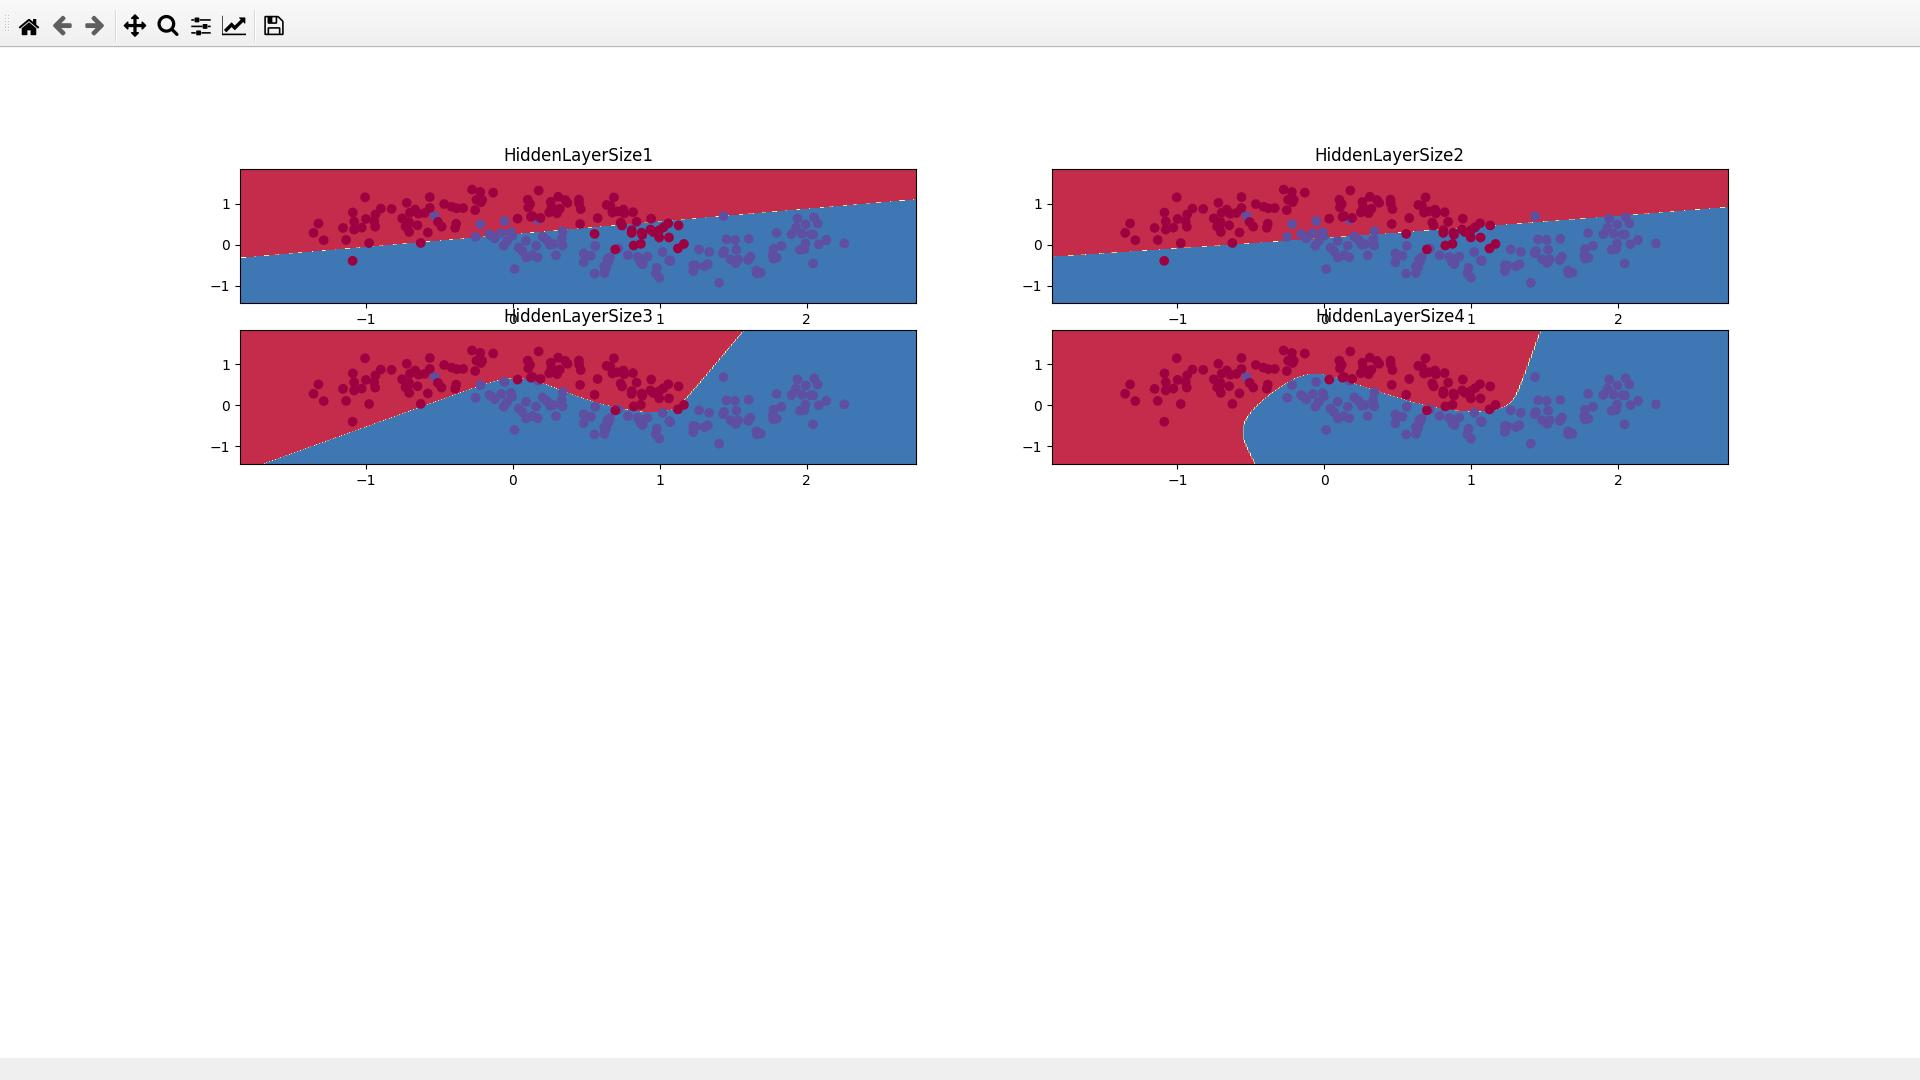
\includegraphics[scale=.25]{plot.jpg}
\end{document}
